\chapter{Introduction}
\vspace*{0.5cm}
\setcounter{page}{1}
\pagenumbering{arabic}

Since the start of 2020 \textit{Sars-COVID19} has initiated a world-wide pandemic. In an attempt to slow down the fast and uncontrollable spread of this disease various prevention and diagnosis methods have been developed. In this work, out of all these various methods, the attention is going to be put on the possible developement diagnostic methods related to medical images, be they automatic or semi-automatic, to be intended either as Clinical Decision Support Systems (CDSS) or as a quick evaluation to completely avoid human analysis.
In this light this first introductory chapter is going to start from a basic theoretical overview of the necessary core concepts that will be needed throughout this whole work such as definition of an image and imaging methods, with particular attention to those used in the medical field. This will be followed by an introduction to Artificial Intelligence (AI) and some Machine Learning techniques. Finally some of the concepts from the two previous topics will be treated jointly under the discipline of radiomics, which will be defined and explored as necessary.

\section{Theoretical background: Medical Images}
In this section the objective is to simply provide a set of basic definitions pertaining to images as well as a general introduction to the methods used to create said images. Firstly images are a means of representing in a visual way a physical object or set thereof, when talking about images it's common to refer specifically to digital images.

\begin{definition}[Digital Image]
A numerical representation of an object; more specifically an ordered array of values representing the amount of radiation emitted (or reflected) by the object itself. The values of the array are associated to the intensity of the radiation coming from the physical object; to represent the image these values need to be associated to a scale and then placed on a discrete 2D grid. 
To store these intensities the physical image is divided into regular rectangular spacings, each of which is called pixel\footnote{The term pixel seems to originate from a shortening of the expression Picture's (pics=pix) Element(el). The same hold for voxel which stands for Volume Element}, to form a 2D grid; inside every spacing is then stored a number (or set thereof) which measures the intensity of light, or color, coming from the physical space corresponding to that grid-spacing. 
The term digital refers to the discretization process that inherently happens in storage of the values, called pixel values, as well as in arranging them within the grid. It's possible to generalize from 2D images to 3D volumes, simply by stacking images of the same object obtained at different depths. In this context, the term pixel is substituted by voxel, however since they are used interchangeably in literature they will, from now on, be considered equivalent.
\end{definition}

Generally pixel values stored as integers p$\in$ [0,2$^{n}$-1] with p,n$\in$ $\mathbb{N}$  or as p$\in$[0,1] with p$\in$ $\mathbb{R}$, the type of value stored within each pixel changes the nature of the image itself. 
A single value is to be intended as the overall intensity of light coming from the part of the object contained corresponding to the gridspace and is used for a gray-scale representation, a set of three\footnote{The three values correspond each to the intensity of a single color, the most commonly used set of colors is the RGB-scale (Red, Green, Blue). Further information can be found by looking into Tristimulus theory\cite{Tristimulus}}  or four\footnote{Same as RGB but with four colors, the most common scale is CMYK (Cyan, Magenta, Yellow, blacK)} values can be intended as a color image.

\begin{figure}[H]
     \centering
     \subfloat[][\centering RGB color space on a cube]{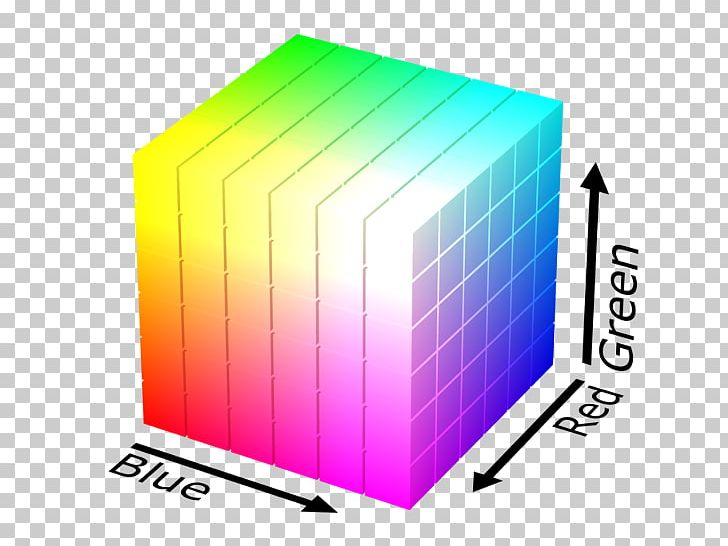
\includegraphics[width=5cm]{RGB_cube.jpg}\label{fig: RGB_cube}}
    \qquad
     \subfloat[][\centering HSV cone]{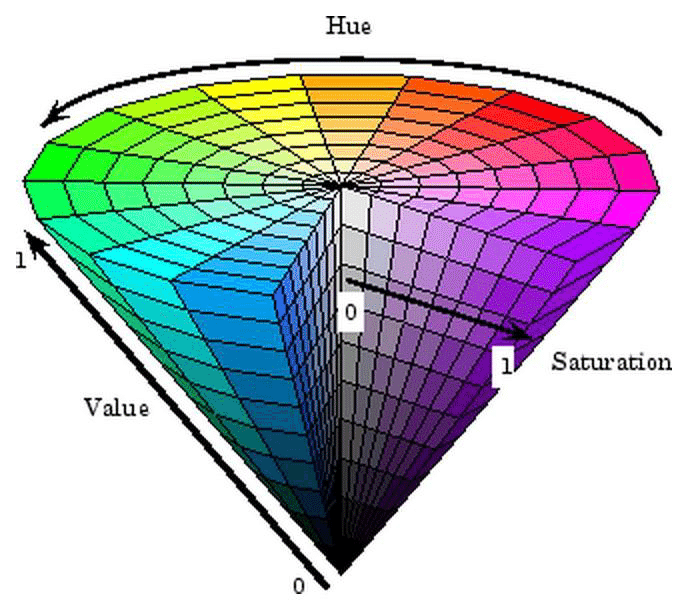
\includegraphics[width=5cm]{HSV_cone.png}\label{fig:HSV_cone}}
     \caption{Examples of color spaces}
     \label{fig:color_spaces}
\end{figure}

There are a lot of possible scales for representation\footnote{Besides RGB and CMYK \ref{fig: RGB_cube} the most common color spaces are CIE (Commision Internationale d’Eclairage) and HSV fig:\ref{fig:HSV_cone} (Hue,Saturation and Value). Refer to \cite{Color_spaces} for further details}, which are sometimes called color-spaces, however the most noteworthy in the scope of this work is the Hounsfield unit (HU) scale.

\begin{definition}[Hounsfield unit (HU)]
A scale used specifically to describe radiodensity, frequently used in the context of CT (Computed Tomography) exams. The values are obtained as a transformation of the linear attenuation coefficient \ref{eq:Lin_att_coef_def} of the material being imaged and, since the scale is supposed to be used on humans, it's defined such that water has value zero and air has the most negative value -1000. For  a more in depth discussion refer to \cite{Hounsfield}
\end{definition}

\begin{equation}\label{eq:HU_def}
    HU = 1000*\frac{\mu - \mu_{H_2O}}{\mu_{H_2O} - \mu_{Air}}
\end{equation}

The utility of this scale is in it's definition, since the pixel value depends on the attenuation coefficient it's possible to individuate a set of ranges that identify, within good reason, the various  tissues in the human body: for example lungs are [-700, -600] while bone can be in the [500, 1900] range.
A more in depth discussion of the topics relative to Hounsfield units is going to be carried out at a later point throughout this chapter, in the meantime it's necessary to clarify what are the most important characteristics of an image:

\begin{itemize}
\item Spatial Resolution: A measure of how many pixel are in the image or, equivalently, how small each pixel is; a larger resolution implies that smaller details can be seen better fig:\ref{fig:resolution_types}. Can be measured as the number of pixel measured over a distance of an inch ppi(Pixel Per Inch) or as number of line pairs that can be distinguished in a mm of image lp/mm (line pair per millimeter).
\item Gray-level Resolution: The range of the pixel values, a classic example is an 8-bit resolution which yields 256 levels of gray. A better resolution allows a better distinction of colors within the image fig:\ref{fig:resolution_types}.

\begin{figure}[H]
  		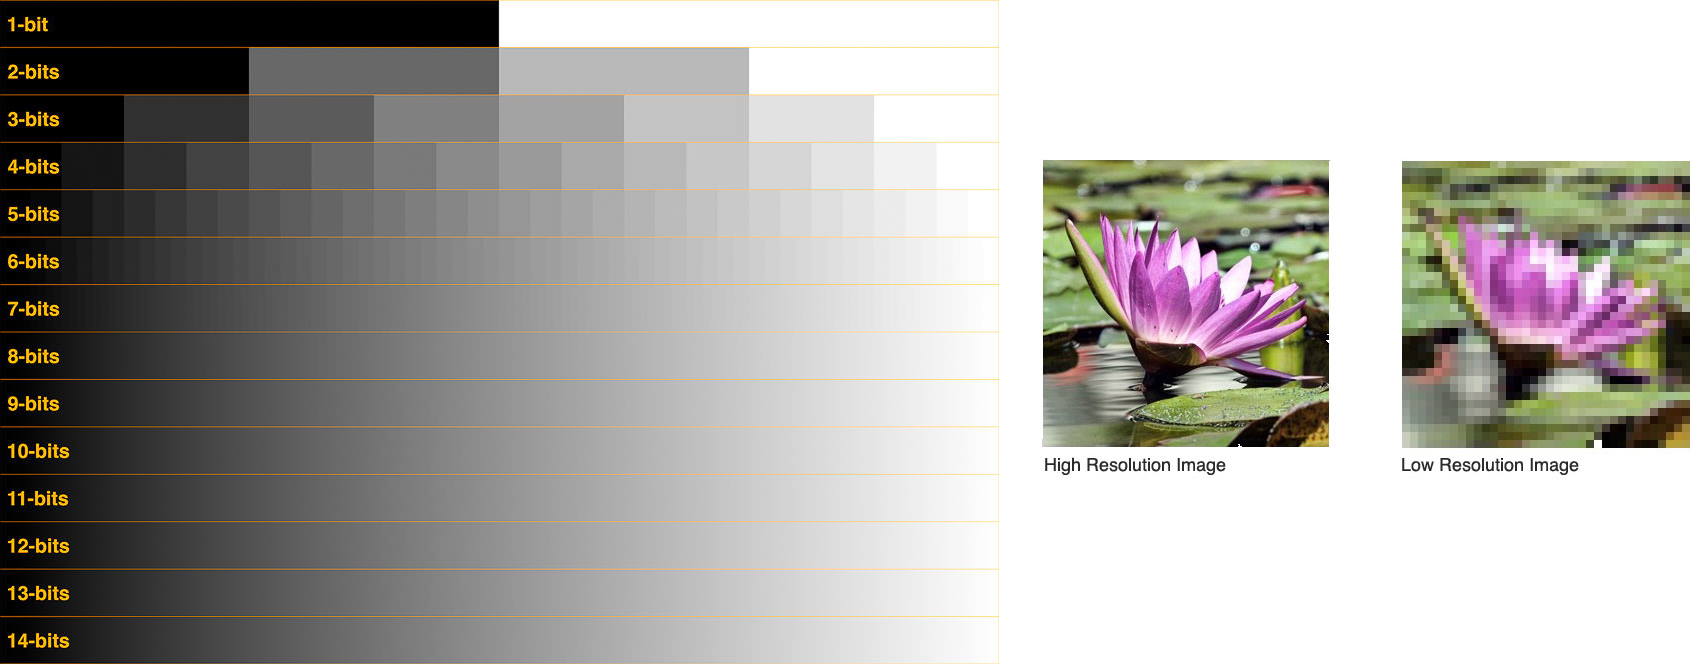
\includegraphics[width=0.8\textwidth]{Img_resolution.png}
        \caption{Example of visual differences in Gray-level (left) and spatial (right) resolution \label{fig:resolution_types}}
\end{figure}

\item Size: Refers to the number of pixel per side of the image, for example in CT-derived images the coronal slices are usually 512x512. These numbers depend on the acquisition process and instrument but in all cases these refer to the number of rows and columns in the sampling grid as well as in the matrix representing the image.
\item Data-Format: How the pixel values are stored in the file of the image. The most commonly used formats are .PNG and .JPG however there are a lot of other formats. In the context of this work, which is going to be centered on medical images, the most interesting formats are going to be the nii.gz (Nifti) and the .dcm (DICOM). The first contains only the pixel value information hence it's a lighter format, it originates in the field of Neuroimaging\footnote{In fact Nifti stands for Neuroimaging Informatics Technology Initiative (NIfTI)}, it is used mainly in Magnetic resonance images of the brain but also for CT scans and, since it contains only  numeric information, it's the less memory consuming option out of the two. The second contains not only the image data but also some data on the patient, such as name and age, and details on how the exam was carried out, such as machine used and specifics of the acquisition routine. This format is heavier than the previous one and, for privacy purposes, is much more delicate to handle which is why anonymization of the data needs to be taken in consideration. For a thorough description of the DICOM standard refer to \cite{DICOM}. 
\end{itemize}

The format in which the image is saved depends on the compression algorithm used to store the information within the file. These algorithms can be lossy, in which case some of the information is lost to reduce the memory needed for storage, or lossless which means that all the information is kept at the expense of memory space. The first set of methods is preferred for storage of natural images, these are cases in which details have no importance, whereas the second set of methods is used where minute details can make a considerable difference such as in the medical field\footnote{A detailed description of compression algorithms is beyond the scopes of this thesis, for this reason please refer to \cite{Img_Compression} for more information}.
Given this set of characteristics it should now be clear that images can be thought of as array of numbers, for this reason they are often treated as matrices and, as such, there is a well defined set of valid operations and transformations that can be performed on them. All these operations and transformations, in a digital context\footnote{As opposed to analog context, which would mean the chemical processes used at the start of photography to develop and modify the film on which the image was stored}, are performed via computer algorithms which allow almost perfect repeatability and massive range of possible operations. 
Given the list-like nature of images one of the most natural things to do with the pixel values is to build an histogram to evaluate some of the characteristic values of their distribution, such as average, min/max, skewness, entropy... . The histogram of the image, albeit not being an unambiguous way to describe images, is very informative. When looking at an histogram it's immediately evident whether the image is well exposed and if the whole range of values available is being used optimally. 

\begin{figure}[H]
  		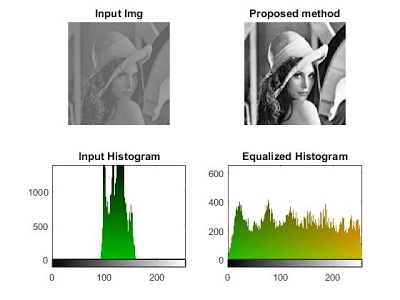
\includegraphics[width=0.8\textwidth]{Contrast_enhancement.jpg}
        \caption{Example of differences in contrast due to histogram equalization\label{fig:contrast_enhancement}}
\end{figure}

This leads us to the concept of \textit{Contrast} which is a quantification of how well different intensities can be distinguished. If all the pixel values are bundled in a small range leaving most of the histogram empty then it's difficult to pick up the differences because they are small however, if the histogram has no preferentially populated ranges then the differences in values are being showed in the best possible way fig:$\ref{fig:contrast_enhancement}$. Note also that if looking at the histogram there are two(or more) well separated distributions it's possible that these also identify different objects in the image, which will for example allow for some basic background-foreground distinction.
Assuming they are being meaningfully used \footnote{For example adding/subtracting one image to/from another can be reasonably understood, multiplying/dividing are less obvious but still used e.g. in scaling/mask imposition and change detection respectively} all mathematical operations doable on matrices can be performed on images for this reason it would be useless to list them all. However, it's useful to provide a list of categories in which transformations can be subdivided:

\begin{enumerate}
\item Geometric Transformations involve the following steps:
		\begin{enumerate}
		\item Affine transformations: Transformations that can can be performed via matrix multiplication such as rotations, scaling, reflections and translations. This step basically involves computing where each original pixel will fall in the transformed image
		\item Interpolation: Since the coordinates of the transformed pixel might not fall exactly on the grid it might become necessary to compute a kind of average contribution of the pixel around the destination coordinate to find a most believable value. Examples of such methods are linear, nearest neighbour and bicubic. 
		\end{enumerate}
\item Gray-level (GL) Transformations: Involve operating on the value stored within the pixel, these can be further subdivided as:
		\begin{enumerate}
		\item Point-wise: The output value at specific coordinates depends only on the output value at those same specific coordinates. Some examples are window-level operations, thresholding, negatives and non-linear operations such as gamma correction which is used in display correction. Taken p as input pixel value and q as output and given a number $\gamma \in \mathbb{R}$, gamma corrections are defined as:
		\begin{equation}
		q = p^{\gamma}
		\end{equation}
		\item Local: The output value at specific coordinates depends on a combination of the original values in a neighbourhood around that same coordinates. Some examples are all filtering operation such as edge enhancement, dilation and erosion. These filtering methods are based on performing convolutions which will be explained in \ref{sec:Convolution}
		\item Global: The output value at specific coordinates depends on all the values of the original images. Most notable operation in this category is the Discrete Fourier Transform and it's inverse which allow switching between spatial and frequency domains. It's worth noting that high frequency encode patterns that change on small scales whereas low frequencies encode regions of the image that are constant or slowly varying.
		\end{enumerate}
\end{enumerate}

The aforementioned is surely not a comprehensive list of all that can be said on images however it should be enough for the scopes of this work.

\vspace{7mm} %7mm vertical space

Having seen what constitutes and image and what can be done with one it becomes interesting to explore how images are obtained. The following discussion is going to introduce briefly some of the methods used to obtain medical images, getting more in depth only on the modality used to obtain all the images used in this thesis which is Computed Tomography.

\begin{enumerate}
\item Magnetic Resonance Imaging (MRI): This technique is based on the phenomenon of Nuclear Magnetic Resonance(NMR) which is what happens when diamagnetic atoms are placed inside a very strong uniform magnetic field are subject to Radio Frequency (RF) stimulus. These atoms absorb and re-emit the RF and supposing this behaviour can somehow be encoded with a positional dependence then it's possible to locate the resonant atoms given the response frequency measured. Suffices to say that this encoding is possible however the setup is very complex and the possible images obtainable with this method are very different and can emphasize very different tissue/material properties. Nothing more will be said on the topic since no data obtained with this methodology will be used. More details can be found in \cite{MRI}
\item Ultra-Sound (US): The images are obtained by sending waves of frequency higher to those audible by humans and recording how they reflect back. This technique is used mainly in imaging soft peripheral tissues and the contrast between tissues is given by their different responses to sound and how they generate echo. The main advantages such as low cost, portability and harmlessness come at the expense of explorable depth, viewable tissues, need for a skilled professional and dependence on patient bodily composition as well as cooperation.
\item Positron Emission Tomography (PET): In this case the images are obtained thanks to the phenomenon of annihilation of particle-antiparticle, specifically of electron-positron pairs.	The positrons come from the $\beta ^+$ decay of a radio-nucleide bound to a macromolecule, which is preferentially absorbed by the site of interest \footnote{Most commonly Fluoro-DeoxyGlucose FDG which is a glucose molecule labelled with a $^{18}$F atom responsible of the $\beta ^+$ decay. In general these radio-pharmaceuticals are obtained with particle accelerators near, or inside, the hospital that uses them. They are characterized by the activity measured as decay/s $\doteqdot$ Bq (read Becquerel) and half-life $\doteqdot$ T$_{\frac{1}{2}}$ which is how long it takes for half of the active atoms to decay}. Once the annihilation happens a pair of (almost) co-linear photons having (almost) the same energy of 511 keV is emitted, the detection of this pair is what allows the reconstruction of the image representing the pharmaceutical distribution within the body. Once again there are a lot of subtleties that are beyond the scopes of this thesis, suffices to say that: firstly the exam is primarily used in oncology given the greater energy consumption, hence nutrients absorption, of cancerous tissue and secondly this technique can be combined with CT scans to obtain a more detailed representation of the internal environment of the patient
\end{enumerate}

The last technique that is going to be mentioned is Computed Tomography however, given it's relevance inside this thesis work, it seems appropriate to describe it in a dedicated section.

\subsection{X-ray imaging and Computed Tomography (CT)}
It's well known that the term x-rays is used to characterize a family electromagnetic radiation defined by their high energy and penetrative properties. Radiation of this kind is created in various processes such as characteristic emission of atoms, also referred to as x-ray fluorescence, and Bremsstrahlung, braking radiation\footnote{From the German terms \textit{Bremsen} "to brake" and \textit{Strahlung} "radiation"}. The discovery that "A new kind of ray"\cite{Roentgen} with such properties existed was carried out by W.C.Roentgen in 1895, which allowed him to win the first Nobel prize in physics in the same year. Clearly the first imaging techniques that involved this radiation were much simpler than their modern counterpart, first of all they were planar and analog in nature, as well as not as refined in image quality. The first CT image was obtained in 1968 in Atkinson Morley's Hospital in Wimbledon. Tomography indicates a set of techniques\footnote{from the greek $\textit{Tomo}$ which means "to cut" and suffix -graphy to denote that it's a technique to produce images} that originate as an advancement of planar x-ray imaging; these techniques share most of the physical principles with planar imaging while overcoming some of it's major limitations, main of which being the lack of depth information.  X-ray imaging, both planar and tomographic, involves seeing how a beam of photons changes after traversing a target, the process amounts to a kind of average of all the effects occurred over the whole depth travelled. 
The way in which slices are obtained is called focal plane tomography and, as the name suggests, the basic idea is to focus in the image only the desired depth leaving the unwanted regions out of focus. This selective focusing can be obtained either by taking geometrical precautions while using analog detectors, such as screen-film cassettes, or by feeding the digital images to reconstruction algorithms to perform digitally the required operations\footnote{In the first case the process is referred to as \textit{Geometric Tomography} while in the second case as \textit{Digital Tomosynthesis}}.
In both planar and tomographic setting the rough description of the data acquisition process can be summarized as follows: First x-rays are somehow generated by the machine, the quality of these x-rays is optimized with the use of filters then focused and positioned such that they mostly hit the region that needs imaging. The beam then exits the machine and starts interacting with the imaged object\footnote{In this work it's always going to be a patient, however this process is general and is also used in industry to investigate object construction}, this process causes an attenuation in the beam which depends on the materials composing the object itself. Having then travelled across the whole object it interacts with a sensor, be it film, semiconductor or other, which stores the data that will then constitute the final image. In a digital setting this final step has to be performed following a (tomographic) reconstruction algorithm which given a set of 2D projections returns a single 3D image.
In this light the interesting processes are how the radiation is created and shaped before hitting the patient and how said radiation then interacts with the matter of both the patient's body and the sensor beyond it. To explore these topics it's necessary to see:
\begin{itemize}
\item How these x-ray imaging machines are structured 
\item How x-ray and matter interact as the first traverses the second
\end{itemize}

It would also be interesting to talk about reconstruction algorithms however since it's beyond the scopes of this work {\Large MAGARI DIRE CHE USEREMO SOLO RICOSTRUZIONI DI UN TIPO QUINDI NON CI INTERESSA VEDERE LE DIFFERENZE?}, refer to \cite{xray_reconstruction} and \cite{PhysicsMedicalImaging}.

\subsubsection{Generation and management of radiation: digital CT scanners}

As of the writing of this thesis, seven generations of CT scanners with different technologies used. The conceptual structure of the machines is mostly the same, and the differences between generations also make evident those between machines. Exploiting this fact the structural description is going to be only one followed by a brief list of notable differences between generations.

\begin{figure}[H]
\centering
  		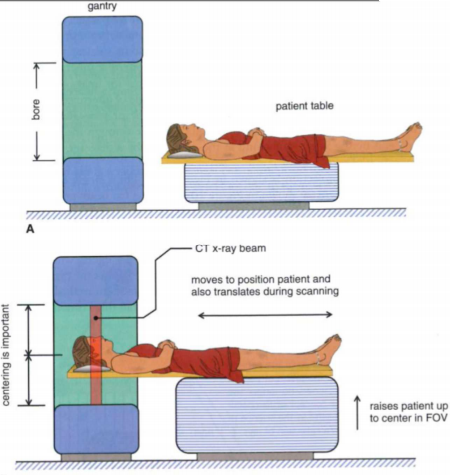
\includegraphics[scale=0.5]{CT_general.png}
        \caption{General set-up of a CT machine\label{fig:CT-machine}}
\end{figure}

The beam is generally created by the interaction of high energy particles with some kind of material, so that the particle's kinetic energy can be converted into radiation. In practice this means that an x-ray tube is encapsulated in the machine. Inside this vacuum tube charged particles\footnote{Most commonly electrons} are emitted from the cathode, accelerated by a voltage differential and shot onto a solid anode\footnote{Typical materials can be Tungsten, Molybdenum}. This creation process implies that the spectrum of the produced x-rays is composed of the almost discrete peaks of characteristic emission, due to the atoms composing the target, superimposed with the continuum Bremsstrahlung radiation.

\begin{figure}[H]
		\centering
  		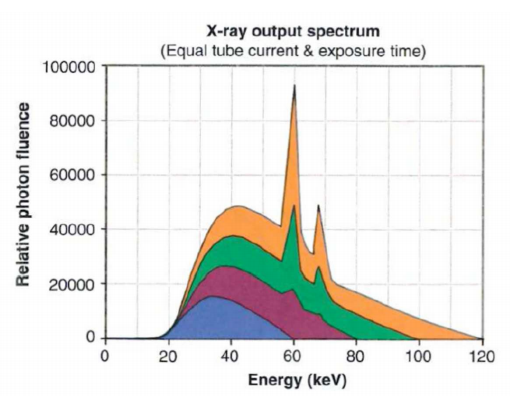
\includegraphics[width=0.8\textwidth]{xray_spectrum.png}
        \caption{X-ray spectrum, composed of characteristic peaks and Bremsstrahlung	continuum, computed at various tube voltages\label{fig:x-ray spectrum}}
\end{figure}

Some of the main characteristics of the x-ray beam are related to this stage in the generation, the Energy of the beam is due to the accelerating voltage in the tube  whereas the photon flux is determined by the electron current in the tube. Worth noting, en passant, that these two quantities can be found in the DICOM image of the exam as \textit{kiloVolt Peak (kVP)} and \textit{Tube current mA} and can be used to compute the dose delivered to the patient.
Other relevant characteristics in the tube are the anode material, which changes the peaks in the x-ray spectrum and time duration of the emission, which is called exposure time and influences dose as well as exposure\footnote{Exposure is a term used to identify how much light has gotten in the imaging sensor. Too high an exposure usually means the image is burnt, i.e. too bright and white, while lower exposures are usually associated to darker images. Exposure is proportional to the product of tube current and exposure time, measured in mA*s. Generally the machine handles the planning of exposure time according to treatment plan}.
The electron energy is largely wasted ($\sim 99\%$) as heat in the anode, which then clearly needs to be refrigerated. The remaining energy, as said before, is converted into an x-ray beam which is directed onto the patient. To reduce damage delivered to the tissues it's important that most of the unnecessary photons are removed from the beam. 
Exploiting the phenomenon of beam hardening a filter, usually of the same material as the anode, is interposed between the beam and the patient to block lower energy photons from passing through thereby reducing the dose conveyed to the patient. At this point there may also be some form of collimation system which allows further shaping of the dose delivered. Having been collimated the beam traverses the patient and gets to the sensor of the machine, which nowadays are usually solid-state detectors.
Naturally the description of these technologies can be done on a much finer level, however for the scopes of this work this description is deemed sufficient {\Large FORSE ANCHE TROPPO? O TROPPO POCO??}
At this point is where the differences between generations arise which,loosely speaking, can be found in the emission-detection configuration and technology.

\begin{itemize}
\item $1^{st}$ generation-Pencil Beam: A single beam is shot onto a single sensor, both sensor and beam are translated across the body of the patient and then rotated of some angle. The process is repeated for various angles. Main advantages are scattering rejection and no need for relative calibration, main disadvantage is time of the exam
\item $2^{nd}$ generation-fan Beam: Following the same process as the previous generation the main advantage is the reduction of the time of acquisition by introducing N beam and N sensors which don't wholly cover the patient's body so still need to translate.

\begin{minipage}{\linewidth}
            \centering
            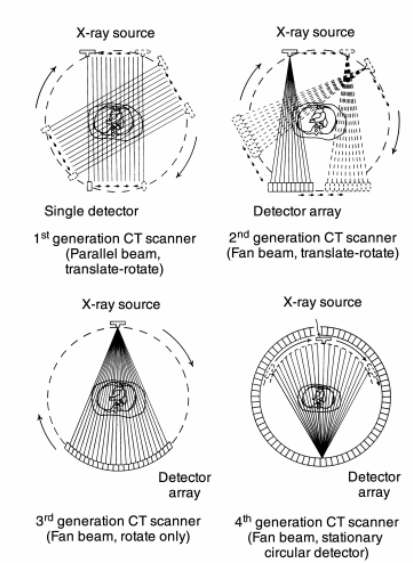
\includegraphics[width=6cm]{CT_gen1.png}
            \captionof{figure}{First four generation of CT scanners}
        \end{minipage}
        
\item $3^{rd}$ generation-Rotate Rotate Geometry: Enlarging the span of the fan of beams and using a curved array of sensor a single emission of the N beams engulfs the whole body so the only motion necessary is rotation of the couple beam-sensor array around the patient.
\item $4^{th}$ generation-Rotate Stationary Geometry: The sensors are now built to completely be around the patient so that only the beam generator has to rotate around the body \newline
\item $5^{th}$ generation-Stationary Stationary Geometry: The x-ray tube is now a large circle that is completely around the patient. This is only used in cardiac tomography and as such will not be described further \cite{Cardiac-CT}
\item $6^{th}$ generation-Spiral CT: Supposing the patient is laying parallel to the axis of rotation, all previous generations acquired, along the height of the patient, a single slice at a time. In this generation as the tube rotates around the patients the bed on which they're laying moves along the rotation axis so that the acquisition is continuous and not start-and-stop. This further reduces the acquisition time while significantly complicating the mathematical aspect of the reconstruction. It's necessary to add another important parameter which is the pitch of the detector\footnote{Once again the important parameters, such as this, can be accessed in the DICOM file resulting from the exam,}. This quantifies how much the bed moves along the axis at each turn the tube makes around the patient. Pitches smaller than one indicate oversampling at the cost of longer acquisition times, pitches greater than one indicate shorter acquisition times at the expense of a sparser depth resolution. \newline
\begin{minipage}{\linewidth}
            \centering
            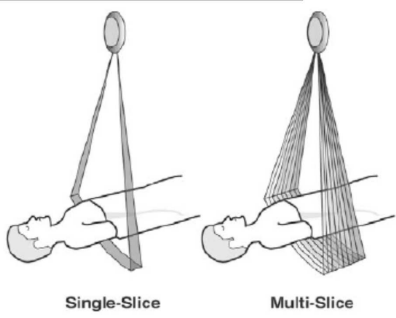
\includegraphics[width=6cm]{CT_gen2.png}
            \captionof{figure}{$7^{th} generation setup$}
        \end{minipage}
\item $7^{th}$ generation-MultiSlice: Up to this seventh generation height-wise slice acquisition was of a singular plane, be it continuous or in a start and stop motion. In this final generation mutliple slices are acquired. Considering cilindrical coordinates with z along the axis of the machine the multiple slice acquisition is obtained by pairing a fanning out along $\theta$ and one along z of both sensor arrays and beam. This technique returns to a start and stop technology in which only $\sim 50\%$ of the total scan time is used for acquisition
\begin{minipage}{\linewidth}
            \centering
            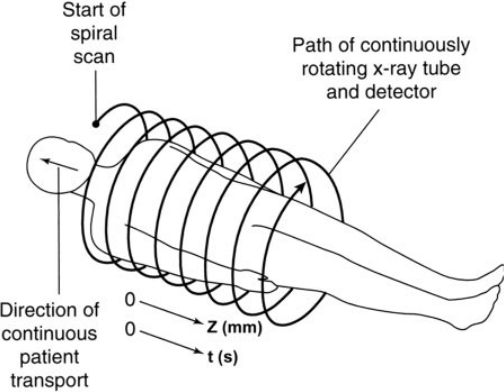
\includegraphics[width=6cm]{CT_gen3.png}
            \captionof{figure}{$7^{th} generation setup$}
        \end{minipage}
\end{itemize}

The machines used to obtain the images used in this thesis, all belonging to the Ospedale S. Orsola, were either spiral CTs or .


\subsubsection{Radiation-matter interaction: Attenuation in body and measurement}
Having seen the apparatus for data collection the remaining task is to see how the information regarding the body composition can be actually conveyed by photons.
Let's first consider how a monochromatic beam of x-rays would interact with an object while passing through it. All materials can be characterized by a quantity called attenuation coefficient $\mu$ which quantifies how waves are attenuated traversing them, this energy dependent quantity is used in the Beer-Lambert law which allows computation of the surviving number of photons, given their starting number $N_0$ and $\mu$:

\begin{equation}
N(x) = N_0e^{-\mu(E)*x}
\label{Beer-Lambert}
\end{equation}

At a microscopic level the absorption coefficient will depend on the probability that a photon of a given energy E interacts with a single atom of material. This can be expressed using atomic cross section $\sigma$ as:

\begin{equation}\label{Lin_att_coef_def}
\mu(E) = \frac{\rho*N_A}{A}*(\sigma_{Photoelectric}(E)+\sigma_{Compton}(E)+\sigma_{PairProduction}(E))
\end{equation}

Where $\rho$ is material density, $N_A$ is Avogadro's number, A is the atomic weight in grams and the distinction among the various possible interaction processes for a generic photon of high energy E is made explicit. Overall the behaviour of the cross section is the following

\begin{figure}[H]
\centering
  		\includegraphics[]{cross_section.png}
        \caption{Photon cross-section in Pb\label{fig:Photon-Cross-sect}}
\end{figure}

Overall, given eq:\ref{Beer-Lambert}, it's clear to see that the attenuation behaviour of a monochromatic beam would be linear in semi-logarithmic scale hence the name for $\mu$ "\textit{Linear Attenuation Coefficient}". The first complication comes from the fact that, given their generation method, the x-rays are not monochromatic but rather polychromatic. This property causes the phenomenon of beam hardening: lower energy x-rays interact much more likely than those at higher energies which implies that as it crosses some material the mean energy of the whole beam increases. This behaviour is exploited still within the machine, filters are interposed between anode and patient to reduce the useless part of the spectrum as shown in fig: \ref{fig:Beam-filtering}:

\begin{figure}[H]
\centering
  		\subfloat[Beam Filtering]{
  		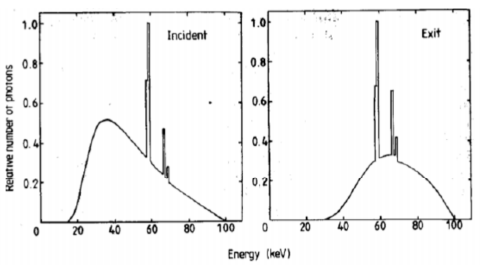
\includegraphics[scale=0.5]{Beam_Filtering.png}
        \label{fig:Beam-filtering}}
        \subfloat[Polychromatic beam attenuation]{
  		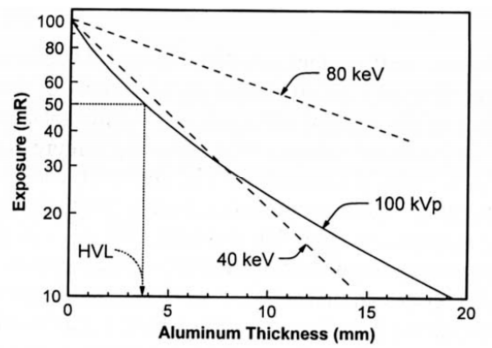
\includegraphics[scale=0.4]{Nonlin_attenuation.png}
        \label{fig:non_lin_attenuation}}
        \caption{Polychromatic beam behaviour}\label{fig:polychrom_behaviour}
\end{figure}

Another effect of the beam being polychromatic is that the graphical behaviour of the attenuation instead of being linear gets bent as shown in fig: \ref{fig:non_lin_attenuation} which is consistent with beam hardening. Since the image brightness is related to the number of photons that get on the sensor it's still possible to define the contrast between two pixel as:

\begin{equation}
C(p1,p2) = \frac{N_{\gamma ,p_2}-N_{\gamma ,p_1}}{N_{\gamma ,p_2}}
\end{equation}

This formula, that connects the beam to the image, together with eq: \ref{Beer-Lambert}, which connects the beam property to the patient's composition, make clear the processes by which the beam carries patient information. Another complication arises in the context of this last equation due to the phenomenon of scattering which reduces the contrast by changing the direction of the bean and introducing an element of noise. Anti-scattering grids are positioned right before the sensors to reduce this effect by allowing to reach the sensor to only the photons with the correct direction.
\newline The biological effects of radiation won't be treated in this thesis. Suffices to say that damage can be classified as primary, due to ionization events within the nucleus of the cell, or secondary, due to chemical changes in the cell environment. The energy deposited per unit mass is called dose and is measured in Gy(Gray) and, as said before, depends on exposure time, current and kVP of the tube. Most of contemporary machines for CT self-regulate exposure time during the acquisition automatically using Automatic Exposure Control(AEC). Having the dose it's possible to estimate the fraction of surviving cells and, to do so, various models are used. To an introduction to one of these models, the Linear Quadratic (LQ) refer to \cite{LQ_model}.\newline 

\section{Theoretical background: Artificial Intelligence (AI) and Machine Learning(ML)}

\subsection{Artificial Neural Networks}
\subsubsection{Convolution}\label{sec:Convolution}

\section{Combining radiological images  with AI: Radiomics}



\begin{equation}\label{eq:1}
    EM=\int n_e^2~dl\approx\left \langle n_e \right \rangle^2l\qquad \mathrm{pc ~cm^{-6}},
\end{equation}

\vspace*{0.8cm}
\begin{table}[H]
    \centering
    \caption{esempio di tabella e label associati \label{tab:param}}
    \label{parametri}
    \begin{tabular}{@{}lllll@{}}
    \toprule
    Class of Region & \begin{tabular}[c]{@{}l@{}}Size\\ (pc)\end{tabular} & \begin{tabular}[c]{@{}l@{}}Density\\ ($\mathrm{cm^{-3}}$)\end{tabular} & \begin{tabular}[c]{@{}l@{}}$EM$\\ ($\mathrm{pc\:cm^{-6}}$)\end{tabular} & \begin{tabular}[c]{@{}l@{}}Ionized Mass\\ ($\mathrm{M_\odot}$)\end{tabular} \\ \midrule
    Hypercompact & $0.03$ & $10^6$ & $10^{10}$ & $10^{-3}$ \\
    Ultracompact & $0.1$ & $10^4$ & $10^7$ & $10^{-2}$ \\
    Compact & $0.5$ & $5\cdot 10^3$ & $10^7$ & $1$ \\
    Classical & $10$ & $100$ & $10^2$ & $10^5$ \\
    Giant & $100$ & $30$ & $5\cdot 10^5$ & $10^3-10^6$ \\
    Supergiant & $100$ & $10$ & $10^5$ & $10^6-10^8$ \\ 
    \bottomrule
    \end{tabular}
\end{table}




